% !TEX TS-program = xelatex
% !TEX encoding = UTF-8 Unicode
% !Mode:: "TeX:UTF-8"

\documentclass{resume}
\usepackage{zh_CN-Adobefonts_external} % Simplified Chinese Support using external fonts (./fonts/zh_CN-Adobe/)
%\usepackage{zh_CN-Adobefonts_internal} % Simplified Chinese Support using system fonts
\usepackage{linespacing_fix} % disable extra space before next section
\usepackage{cite}
\usepackage{graphicx} % import graphicx, display images
\usepackage{tabularx} % import tabularx, use tables 
\usepackage{makecell}
\usepackage{amsmath}
\usepackage{pifont}


\usepackage{fancyhdr} % 页脚包
\renewcommand{\today}{\number\year/\number\month/\number\day}
\fancypagestyle{stylex}{
\fancyhf{}
\lfoot[L]{\textsc{\today}}	%左侧页脚
%\cfoot{\textsc{\thepage/\pageref*{LastPage}}}	%中间页脚
\cfoot{\textsc{\thepage/4}}
\rfoot[R]{\copyright~2024 {\small 个人简历\ding{118}尚祚彦}}	%右侧页眉
\renewcommand{\headrulewidth}{0pt}
%\renewcommand{\footrulewidth}{1pt}
}
\pagestyle{stylex} % 应用页眉页脚定义

\title{尚祚彦的简历}
\date{\today}
\author{Roy Zuoyan Shang}






\begin{document}
\pagenumbering{arabic} % page number

% \firstname{Roy}
% \familyname{Shang}
%\name{尚祚彦}
%\title{Resum\'{e}}
% \address{紫东路18号}{210046, 南京}
%\phone{(+86) 13913834668}
%\email{shangzuoyan@hotmail.com}
%\homepage{homepage (optional)}



%\maketitle

\begin{table}[!ht]
\flushleft
\begin{tabular}{lc}
\begin{minipage}{0.20\columnwidth}
    \flushleft
    {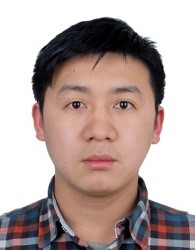
\includegraphics[width=0.8\textwidth]{./images/00.jpg}}
\end{minipage}& \begin{minipage}{.76\textwidth}\raggedright
  \pinfo{尚祚彦 | Roy(Zuoyan)Shang}{1981/01/26,南京}\leavevmode\\
  \wwwinfo{(+86) 13913834668}{shangzuoyan@hotmail.com}{https://shangzuoyan.github.io}
  \end{minipage}
\end{tabular}
\end{table}

% 00::Avatar
%\begin{figure}[htbp]
%      \flushleft
%      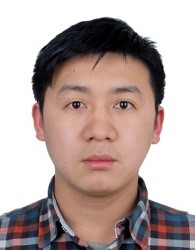
\includegraphics{./images/00.jpg}
%\end{figure}



%\name{尚祚彦}
%\phone[mobile]{(+86) 13913834668}
%\email{shangzuoyan@hotmail.com}
%\url{https://shangzuoyan.github.io/}
% {E-mail}{mobilephone}{homepage}
% be careful of _ in emaill address
% \contactInfo{(+86) 13913834668}{shangzuoyan@hotmail.com}{软件工程师}{GitHub @shangzuoyan}
% {E-mail}{mobilephone}
% keep the last empty braces!
% \contactInfo{shangzuoyan@hotmail.com}{(+86) 13913834668}{}



 
\section{自我评价 | Self-assessment}
\begin{itemize}
  \setlength\itemsep{0.2ex}
  \item 熟练运用\textsc{C}, \textsc{C++}, \textsc{C\#}, \textsc{Java}, \textsc{Python}和 {\LaTeX} 语言;
  \item 熟悉\textsc{L4}微内核(\textsc{SeL4}/ \textsc{L4Re})以及\textsc{QNX}/ \textsc{HelenOS}等微内核操作系统;
  \item 熟悉\textsc{Hypervisor}虚拟化和\textsc{LXC}容器;
  \item 熟悉\textsc{Linux}/ \textsc{Android}和主流\textsc{RTOS}(\textsc{FreeRTOS}/ \textsc{RT-Thread}/ \textsc{Nucleus});
  \item 熟悉\textsc{TCP}/\textsc{IP}族协议,网络编程和精通设计模式;
  \item 具有良好的系统架构设计能力和嵌入式系统的程序开发经验;
  \item 较强的表达能力,职业级英语能力,有境外工作经验;
  \item 为人诚恳,工作踏实,有较强的学习能力和合作精神;
  \item 健康,开朗,有责任心。
\end{itemize}
\hspace*{1.4em} \textbf{现任职于中汽创智。}
\spaceline{}

% \section{\faGraduationCap\ 教育背景}
\section{教育 | Education}
\datedsubsection{\textbf{南京师范大学},地图学与地理信息系统|电子信息科学类,\textit{理学硕士}}{\textbf{2006.09 - 2009.06}}
\textbf{Cartography and Geographic Information Systems (Master of Science)}\\
School of Geographical Sciences, \textbf{Nanjing Normal University (NJNU)}
\datedsubsection{\textbf{江苏大学},工业设计工程|机械电子类,\textit{工学学士}}{\textbf{1999.09 - 2003.07}}
\textbf{Industrial Design Engineering (Bachelor of Engineering)}\\
School of Mechanical Engineering, \textbf{Jiangsu University (JSU)}
\spaceline{}

% \section{\faCogs\ IT 技能}
%\section{技能 | Skills}
% increase linespacing [parsep=0.5ex]
%\begin{itemize}[parsep=0.2ex]
%  \item \textbf{编程语言}: C, C++, C\#, Java, Python, Shell
%  \item \textbf{操作系统}: Linux/Redhat, SeL4/L4Re/HelenOS, FreeRTOS/RT-Thread/Nucleus/QNX
%  \item \textbf{关键词}: \textsc{GDB(Gef)}, \textsc{OllyDbg}, \textsc{Lauterbach Trace32}, \textsc{ARM}, \textsc{RSIC-V}, \textsc{QEMU}, \textsc{Gem5}
%\end{itemize}

% \end{itemize}
\spaceline{}

\section{工作经历 | Work Experience}
% E:1============================================================
%\datedsubsection{\textbf{中汽创智科技有限公司 [CAIC]}, 基础软件部经理 / 操作系统专家}{\textbf{2021.06-至今}}
\expblockcn{2021.06-至今}{基础软件部经理 / 操作系统专家}{中汽创智科技有限公司 [CAIC]}{智能网联事业部 / 基础软件部}
\expitemcn{
\begin{itemize}
  \item \textbf{全面负责基础软件开发部操作系统的设计研发工作,包括:}\\
  \textsc{CAIC OS} / \textsc{CAIC Hybrid OS} / \textsc{CAIC Hypervisor} / \textsc{CAIC Hypervisor Light} 等产品线的设计研发工作;\\
  \textsc{NXP i.MX8QM} / \textsc{TI TDA4} / \textsc{MTK8675} 平台适配工作。
  \item \textbf{部分联合研发项目:}\\
  负责\textsc{Siemens} / \textsc{Mentor Graphics Nucleus} 合作项目的系统重构设计研发以及认证工作;\\
  负责中瓴智行虚拟化系统\textsc{Raite Hypervisor}合作项目的系统设计研发工作;\\
  负责\textsc{Renesas RH850}/\textsc{U2A}/ \textsc{U2B}的轻量级虚拟化系统项目的系统设计研发以及认证工作;\\
  负责车身控制域基于轻量级虚拟化方案上的\textbf{Zonal}架构\textsc{AUTOSAR CP}系统;\\
  负责地平线机器人J3/ J5辅助自动驾驶操作系统合作项目的系统设计研发工作。
\end{itemize}
}
\par
\textbf{内存}\hspace{2.2em}\textbf{页表}\hspace{2.1em}\textsc{TLB}\hspace{2em}\textbf{中断}\hspace{2em}\textbf{进程}\hspace{2.1em}\textsc{IPC}\\
%\textsc{ARM}\hspace{2em}\textsc{RSIC-V}\\
\textsc{UART}/ \textsc{SPI}/ \textsc{I2C}\hspace{2em}\textsc{CAN}/ \textsc{CANFD}\hspace{2em}\textsc{Ethernet PHY}/ \textsc{MAC}\hspace{2em}\textsc{Connectivity}\& \textsc{Networks}\\
\textsc{GDB(Gef)} \textsc{OllyDbg} \textsc{QEMU}/ \textsc{Gem5}\hspace{1.9em}\textsc{Lauterbach Trace32} 
\spaceline{}

% E:2============================================================
%\datedsubsection{\textbf{富智康集团(南京)通讯有限公司[FIH Communications]},专理课长}{\textbf{2017.10-2021.01}}
\expblockexcn{2017.10-2021.01}{专理 / 课长(师-8级)}{富智康集团(南京)通讯有限公司 [FIH Communications]}{A次-IDM3-NJDC / 连接与协议课}
\expitemcn{
\begin{itemize}
  \item \textbf{全面负责{Sharp}(SG1/ HD1/ VGO/ VG2){Nokia}(ROO/ TAS)项目:}\\
精通\textsc{WLAN}/ \textsc{Bluetooth}/ \textsc{FM}/ \textsc{GNSS},\textsc{NFC}/ \textsc{Felica},\textsc{IR} 等子系统及模块;\\
参与\textsc{Apple}苹果公司\textsc{ICAR Connectivity} 交互场景研发;\\
参与\textsc{Byton}拜腾智慧座舱联合研发工作。
  \item \textbf{部分外包业务:} \\
负责\textsc{Vivo Khronos}项目的无线通信相关子系统的设计研发以及认证工作;\\
负责\textsc{Xiaomi D1S OTA} / \textsc{J15s}项目的无线通信相关子系统的设计研发以及认证工作;\\
负责\textsc{LG DH0}项目的无线通信相关子系统的设计研发以及认证工作。
\end{itemize}
}
\spaceline{}

% E:3============================================================
%\datedsubsection{\textbf{江苏润和软件股份有限公司 | HopeRun},智能终端事业本部,终端OS业务条线 技术总监}{\textbf{2016.01-2017.10}}
\expblockexcn{2016.01-2017.10}{专家级软件工程师 / 技术总监}{江苏润和软件股份有限公司 [HopeRun]}{智能终端事业本部 / 终端OS业务条线}
\expitemcn{
  \begin{itemize}
    \item \textbf{承接{Huawei}中央软件院欧拉实验室{AtelierOS}项目:}\\
    \textsc{AtelierOS}是基于\textsc{L4}微内核的虚拟容器,其上可部署运行多个操作系统并进行无缝切换。\\
    负责系统整体架构设计和实现,适配\textsc{Huawei Mate}系列的演进。
    \item \textbf{承接{Huawei}终端公司Texas AT\&T项目:}\\
    基于\textsc{Qualcomm MSM8939}平台,项目技术负责人,负责系统\textsc{Bringup},认证工作以及问题跟踪。 
    \item \textbf{承接{Huawei}终端公司VR项目:}\\
    负责项目的系统架构和设计,负责关键子系统的开发和编码工作。\\
    基于重构\textsc{gSOAP}的\textsc{OnVIF}服务,基于\textsc{Libevent}的进程间通信服务,以及基于\textsc{Sqlite}的\textsc{DAL}封装。
    \item \textbf{承接{ClouderSemi}公司Smart Watch Turnkey项目:}\\
    负责项目的系统架构和设计,负责基于蓝牙的系统框架开发和编码工作。\\
    基于\textsc{Bluetooth LE}的信令交互私有协议,基于\textsc{Bluetooth RF-COMM}的传输服务,以及\textsc{Bluetooth HFP}/ \textsc{A2DP}的音频服务。
  \end{itemize}
}
\spaceline{}

% E:4============================================================
%\datedsubsection{\textbf{宇龙计算机通信科技(深圳)有限公司},南京研究所-第52部,主任软件工程师}{\textbf{2013.05-2016.01}}
\expblockexcn{2013.05-2016.01}{主任软件工程师}{宇龙计算机通信科技(深圳)有限公司 [Yulong / Coolpad]}{南京研究所 / 第52部}
\expitemcn{
\begin{itemize}
  \item \textbf{酷派海外市场产品研发:}\\
  主要负责\textsc{Connectivity}相关模块:\\
\parbox[t]{3em}{\textbf{WCN:}} \parbox[t]{\textwidth-6em}{
  负责\textsc{WLAN}/\textsc{Bluetooth}/\textsc{FM} 集成芯片\textsc{WCN36\underline{X}0}\{1/ 2/ 6\}的\textsc{Bringup};\\
  相关模块功能开发,认证测试(\textsc{WFA}/\textsc{BQB}, \textsc{BT-IOT}等)问题解决;
  海外运营商相关需求的沟通,以及海外场测问题的快速解决。
}\\

\parbox[t]{3em}{\textbf{GNSS:}} \parbox[t]{\textwidth-6em}{
  \textsc{RF Bringup}工作,包括:\textsc{WTR1605L}/ \textsc{WTR4905 Transceiver},\textsc{SKY65611-11 PA}(\textsc{eLNA})芯片的配置,解决\textsc{AGPS}测试以及\textsc{SUPL1.1}/ \textsc{2.0}认证测试中的问题。
}\\

\parbox[t]{3em}{\textbf{NFC:}} \parbox[t]{\textwidth-6em}{
  \textsc{NXP} \textsc{PN544}/ \textsc{PN547}芯片的\textsc{Bringup},驱动调试,\textsc{NFC}协议栈升级,\textsc{SmartCard}方案集成,
  支持\textsc{EMVCo2.3.3}认证,支持\textsc{VISA}/ \textsc{MASTERCARD}/ \textsc{AMEX}支付功能。
}\\

\parbox[t]{3em}{\textbf{IR:}} \parbox[t]{\textwidth-6em}{
  \textsc{ABOV MC96FR116CU}芯片的\textsc{Bringup},驱动调试工作。\\
  完成\textsc{TMO}运营商新需求的开发工作,包括\textsc{DeviceReporting},\textsc{HW Encyption},\textsc{Anti-theft}等。 
}
  \item \textbf{涉及相关平台产品如下:}\\
\hspace*{3em} MSM8926 (\textsc{Vodafone Smart 4 Max}) / MSM8916 (\textsc{Panasonic ELUGA L 4G}) /\\ 
\hspace*{3em} MSM8909 (中国移动\textsc{China Mobile Y75}) / MSM8939 (奇酷\textsc{Qikoo})等。
\end{itemize}
}
\spaceline{}

% E:5============================================================
%\datedsubsection{\textbf{信源通科技有限公司 [TeleEpoch]},南京研究所-软件部,资深软件工程师/软件部副经理}{\textbf{2009.10-2013.05}}
\expblockcn{2009.10-2013.05}{资深软件工程师 / 软件部副经理}{信源通科技有限公司 [TeleEpoch]}{南京研究所 / 软件部}
\expitemcn{
  \begin{itemize}
    \item \textbf{高通 AMSS8960/AMSS8625 项目:}\\
    \textsc{AMSS8960}:\textsc{G6611}/ \textsc{G3617}项目 / \textsc{AMSS8625}:\textsc{QRD-G2616}/ \textsc{G3616}/ \textsc{G3617}项目\\
主要负责\textsc{Modem}侧软件,承担\textsc{Android Framework}/ \textsc{RIL}、\textsc{QCRIL}层\textsc{Telephony}相关代码实现。
    \item \textbf{高通 AMSS7627 F3610/F3611 项目:}\\
主要负责\textsc{Modem}侧软件,负责\textsc{Android Framework}/ \textsc{RIL}、\textsc{QCRIL}层相关代码实现,负责\textsc{IOT Level2}测试(美国沃斯堡诺西网络实验室)。
    \item \textbf{高通 QSC6085 CDMA 1x EVDO M600项目:}\\
(驻美1年)主要负责\textsc{MMS}、\textsc{WAP}浏览器、\textsc{WWW}(\textsc{Full HTML})浏览器,负责\textsc{MMS}/ \textsc{WAP IOT}测试(美国沃斯堡摩托罗拉网络实验室),与\textsc{PCD},\textsc{UMX}以及\textsc{US Cellular}讨论功能需求和技术支持事宜。
    \item \textbf{高通 QSC6055 CDMA 1x WMDP项目:}\\
主要负责自动语音识别[\textsc{ASR}](科大讯飞\textsc{iFlyTek}/ \textsc{VoiceSignal Tech})和重力传感器[G-Sensor]应用模块,参展\textsc{CES2010}和亚洲电信展。
    \item \textbf{高通 QSC6270 GSM/WCDMA (DSDS)项目:}\\
承担底层驱动工作,包括:
\ding{172} \textsc{FLASH}驱动(\textsc{Micron}/ \textsc{Hynix}),
\ding{173} \textsc{LCD}/ \textsc{MDP}驱动(松瑞\textsc{Sunrise}/ 信利\textsc{Truly}等,\textsc{LCM}驱动\textsc{IC}包括:\textsc{TM2.0 3.55 ILI9341 9225 9225G HX8340B 8347D}),
\ding{174} \textsc{T9}键盘/ \textsc{QWERTY}键盘驱动,\ding{175}\textsc{HALL}器件驱动调试以及\ding{176}\textsc{GSDI}双卡支持的底层实现工作;\\
承担OEM接口封装层以及应用层的工作;\\
负责短信(\textsc{GSM 03.38}/ \textsc{03.40}/ \textsc{07.05}),彩信(\textsc{TS23.140}/ \textsc{OMA}),\textsc{STK}(\textsc{GSM 11.14}),\textsc{SIM}卡(\textsc{TS 31.102}),蓝牙,\textsc{Brew JavaVM},\textsc{WWW}(\textsc{Full HTML})浏览器,多媒体和输入法引擎。
    \item \textbf{高通 MDM6085 CDMA 1x EVDO D2/D3/D5数据卡项目:}\\
主要负责下位机\textsc{AT}命令和上位机同步及拨号软件的开发调试任务。
  \end{itemize}
}
\spaceline{}

% E:6============================================================
%\datedsubsection{\textbf{虚拟地理环境重点实验室[VGEKL]},南京师范大学 / 地理科学学院,研究生}{\textbf{2006.07-2009.05}}
\expblockcn{2006.07-2009.05}{研究生}{虚拟地理环境重点实验室 [VGEKL]}{南京师范大学 / 地理科学学院}
\expitemcn{
  \begin{itemize}
    \item \textbf{基于非流形理论的地下空间实体三维GIS关键技术研究}\\
项目编号:\textsc{2007AA12Z236} [国家863项目][2007.11–2009.05]\\
从事三维\textsc{GIS}框架建设(\textsc{OSGi RCP}框架)、空间数据索引(通用搜索树\textsc{GiST}、空间索引库\textsc{Space Index Library}、混合索引\textsc{OR-}树的算法实现和应用)、数据可视化(\textsc{Open Inventor}, \textsc{IRRLicht}, \textsc{OSG}, \textsc{Coin3D})方面的研究,负责原型系统的开发任务。

  \item \textbf{GIS矢量数据产品版权保护的关键技术研究}\\
项目编号:\textsc{2006AA12Z222} [国家863项目][2006.10–2007.03]\\
从事伪随机序列密钥掩码(\textsc{M}序列,\textsc{Golden}序列以及混沌序列),水印嵌入和提取,小波分解与重构方面的研究,对高维空间数据进行水印嵌入,以达到保护空间数据的目的,参与完成原型系统的开发任务。
\end{itemize}
}
\spaceline{}

% E:7============================================================
%\datedsubsection{\textbf{夏新电子股份有限公司[AMOI]},南京研究院 / 通讯事业部,软件工程师}{\textbf{2003.10-2006.08}}
\expblockcn{2003.10-2006.08}{软件工程师}{夏新电子股份有限公司 [AMOI]}{南京研究院 / 通讯事业部}
\expitemcn{
  \begin{itemize}
    \item \textbf{相关平台和操作系统:}\\
展讯(\textsc{Spreadturm})平台 \textsc{X-Thread}系统;\\
高通(\textsc{Qualcomm})平台 \textsc{Rex} OS / \textsc{Brew} / \textsc{BrewMP}系统;\\
东芝(\textsc{Toshiba})平台 \textsc{iTRON}系统。
    \item \textbf{项目中职责:}\\
主要负责各平台\textsc{Feature Phone}和\textsc{PHS}软件开发,\textsc{MMI}、\textsc{LCD}驱动以及功能业务模块(\textsc{PIM} /\textsc{PIN}模块、电话簿模块和日程安排模块)应用程序的开发任务。\\
积累了丰富的项目开发经验,熟悉了\textsc{PIM}的协议和文件结构,对\textsc{iTRON}系统有了深入的了解。并且在\textsc{PHS S368}项目中担任软件负责人。
  \end{itemize}
}
\spaceline{}
\spaceline{}
\spaceline{}
\spaceline{}

% ============================================================
\section{论文和专利 | Publications and Commitments}
% increase linespacing [parsep=0.5ex]

\textbf{相关论文}

[1] Xu H, Lu G, Sheng Y, Guo F, \textbf{Shang Z}.3D GIS spatial operation based on extended Euler operators[J].\\
  Proceedings of SPIE - The International Society for Optical Engineering, 2008, 7143:71433D-71433D-10.\\
  DOI:10.1117/12.812655.

[2]\textbf{尚祚彦}.3D GIS混合空间索引技术研究[D].南京师范大学,2009.DOI:10.7666/d.d183065.

[3]张璐,柴燕妮,王丹,\textbf{尚祚彦}.基于地理国情的县域生态环境质量评价研究[J].地理空间信息, 2022, 20(10):79-81.
~\\

\textbf{相关专利}
\vspace{0.6ex}{}

\setlength{\extrarowheight}{0.8ex} %设置行高
\begin{tabularx}{\textwidth }{ m{7.2em}|X|m{6.6em}}
\hline
{专利公开号} & {专利描述} & {公开日期}\\
\hline
CN115480934A & 专利一种分布式数据处理的方法、装置、设备及储存介质 & 2022/12/16\\
\hline
CN114153560A & 专利一种虚拟中断处理方法、装置、设备及介质 & 2022/03/08\\
\hline
CN114579556A & 专利一种数据处理方法、装置、设备及存储介质 & 2022/06/03\\
\hline
CN114579556B & 专利一种数据处理方法、装置、设备及存储介质 & 2022/08/02\\
\hline
CN114298990A & 专利一种车载摄像装置的检测方法、装置、存储介质及车辆 & 2022/04/08\\
\hline
CN114500408A & 专利一种以太网络交换装置、数据处理装置和车辆 & 2022/05/13\\
\hline
\end{tabularx}




  
  


%% Reference
%\newpage
%\bibliographystyle{IEEETran}
%\bibliography{mycite}
\end{document}
